\subsection{Choosing the type of pattern}

In the test-1 we can see the correlation analysis of 3 types of patterns
(see Fig. \ref{fig:samplesabc}). This results can be used to select the best pattern
to use in the  load and break study of beams; for example, following the 
Figs. \ref{fig:choosingt16}, \ref{fig:choosingt32} and \ref{fig:choosingt64},
is easy to see that a periodic pattern as $PB$ has also a periodic behavior
in the $PCC$ value; so that we have that consider values of threshold $T \geq 0.82$ 
in the Figs. \ref{fig:choosingt32} and \ref{fig:choosingt64} and $T \geq 0.90$
in the Fig. \ref{fig:choosingt16}, so that
less values of these threshold have the probability of causing false positives in the recognition of an 
analysis region. Given that, in the pattern $PB$, many positions share correlation values with similar values
for a threshold relatively high like $T=0.75$, we not recommend to use periodic patterns like $PB$.

The patterns $PA$ and $PC$ are random in nature, with the difference
that the pattern points in $PC$ are big  and few, and in the $PA$
are many and small. Following the 
Figs. \ref{fig:choosingt16}, \ref{fig:choosingt32} and \ref{fig:choosingt64},
we can see that the $PCC$ values have a behavior approximately monotone decrescent
when the size of analysis region is greater when compared to the size of points
in the pattern. Thus, the pattern $PA$ and $PC$ have a strange behavior to a $WSIZE=16$;
so that the $T$ value, necessary to have  a false positive is
$T<0.60$ to $PA$ and $PC$; we can see this clearly in the Fig. \ref{fig:choosingt16} 
given that the values of $PCC$ that fulfill this condition only are very close to the origin.
In the same sense to a value $WSIZE = 32$, 
the threshold conditions necessary to have  false positives
are $T<0.2$ and $T<0.4$ to $PA$ and $PC$, respectively; these values of $PCC$ are much lower 
and close to the origin therefore never lead to confusion.
Finally, to a  value $WSIZE = 64$, 
the threshold conditions necessary to have  a false positive 
are $T<0.3$ and $T<0.2$ to $PA$ and $PC$, respectively; 
these values of $PCC$ are lower like the one obtained with $WSIZE = 32$,
therefore these are equally convenient to those obtained with $WSIZE = 32$.
Thus, in the Figs. \ref{fig:choosingt16}, \ref{fig:choosingt32} and \ref{fig:choosingt64},
there is not a clear advantage of $PA$ over $PC$ given that both support analysis regions
of $WSIZE \geq 32$.

In the test-2 we can see the correlation analysis of two rotated analysis regions, 
to the 3 types of patterns seen in the Fig. \ref{fig:samplesabc}.
For a fair comparison, we establish the value $PCC=0.82$ as the analysis line to the
Figs. \ref{fig:choosingr16}, \ref{fig:choosingr32} and \ref{fig:choosingr64}, 
given that we consider that
values lower this given us an error in the recognition of the analysis region.
In the Figs.  \ref{fig:choosingr16} and \ref{fig:choosingr32} there is
a marked difference  to recognize an analysis region in favor to the
pattern $PC$, given that this support a superior rotation angle range. Additionally,
in the Fig. \ref{fig:choosingr64} we observe that there is not a 
significant difference between the angle range  when the patterns
$PA$ and $PC$ are compared.
Here, it is important  to note
that in all cases an analysis region with a very large $WSIZE$,
 when compared to the size of the points in the pattern
 (in this case $WSIZE=64$ ), prevents identifying the rotated analysis region correctly.
 This is expected given that 
the deviation to a distance $d_0$ caused by an angle $\alpha_0$ is less significant that
a deviation to a distance $2d_0$. The effect of the rotation is very important 
in the  load and break study of beams, given that in these tests
there are small angle rotations in regions analyzed between to consecutive images.

Thus, we recommend the use of patterns such as $PC$ (with big dot patterns) 
given that to analysis regions, rotated a small angle,
these hold better the $PCC$ value; and consequently the correlation analysis 
is able to identify better a rotated region. 

\subsection{Choosing the window size}

As can be seen in the Test-1, the value of $WSIZE$
influences the recognition of displaced analysis regions.
Thus, a pattern such as $PC$, with patterns points of 
$5$ pixels of diameter and separation of $11$ pixels,
needs  a $WSIZE > 32$ to avoid false positives in the 
analysis region recognition process using a threshold value relatively 
lower, see Fig \ref{fig:choosingt32};
given that, analysis regions with $WSIZE \leq 32$ results in regions with a few
characteristic details (information) and the probability of
finding a similar region is high.

On the other hand as can be seen in the Test-2, the value of $WSIZE$
also influences the recognition of rotated analysis regions.
So that, for a pattern as $PC$, a $WSIZE=64$ only allows
recognition of analysis regions rotated at most a angle of $2.5^\circ$
(for a threshold of $PCC=0.82$). 
Thus, to a pattern like $PC$ (similar diameter and separation of pattern points), 
we recommend to use  a $32 \leq WSIZE \leq 64$.


\subsection{Choosing the threshold value}

For a pattern as $PC$, the choice of a threshold $T$
depends on the used value for $WSIZE$; for example, in the Fig. 
\ref{fig:choosingt16}, 
where is used a $WSIZE=16$,  
the form of the correlation curve limits the threshold
to a value of $T \geq 0.60$, given that smaller values
cause false positives in the recognition process of analysis regions.
Furthermore in the Fig. \ref{fig:choosingt32}
the correlation curve limits the threshold
to a value of $T \geq 0.40$. In all these cases, the specific used 
threshold value of $PCC$ will chosen
taking into account the chosen step length $l_0$.


\subsection{Choosing the step length}
\label{subsec:steplength}

The first thing to consider is that if we define a step length such
as $l_0$ pixels, the maximum (bi-dimensional) measure error, 
in predicting the displacement of an analysis region between two consecutive images,
will be of $l_0\sqrt{2}/2$ pixels. Thus if the step length is $l_0=1$ pixel, then
the maximum displacement error will be of $0.70711$ pixels; being this the minimum
(desirable) of the maximum displacement error in the technique, and we recommend
the use of image sizes that allow acceptable processing times with a step length of
$l_0=1$ pixel. But if is desired to use other values to the step length,
we should take in consideration other involve variables such as the used threshold.

For example, if we establish the threshold for a value of $PCC=0.67$ in the
test-1, where a $WSIZE=32$ is used
(see Fig. \ref{fig:choosingt32zoom}),
then we observe that, for the pattern $PC$, the error in the displacement prediction before
losing the analysis region in the recognition process, it is of $2$ pixels,
or in others words $l_0\sqrt{2}/2 \leq 2$ pixels.
\begin{figure}[H]
\centering
  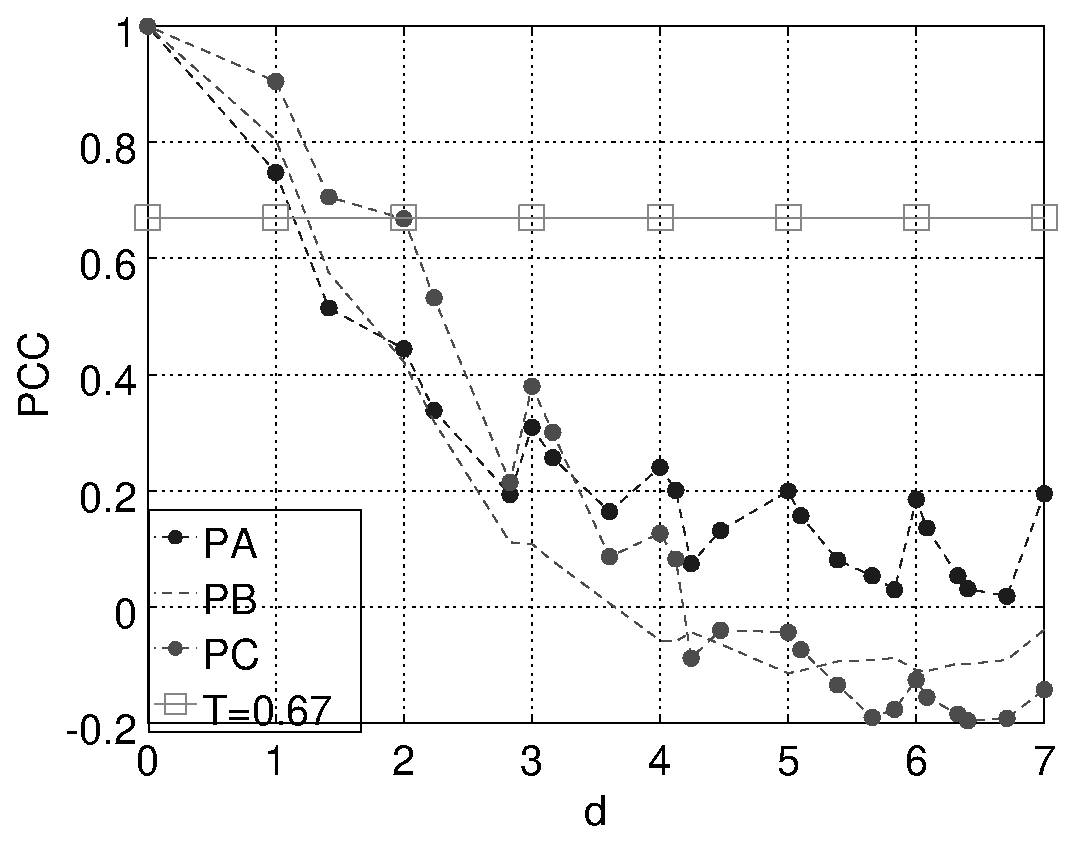
\includegraphics[width=.7\columnwidth]{image_plot-32zoom.eps}
  \caption{Region of analysis with a $WSIZE=32$ and a threshold of $0.67$.}
  \label{fig:choosingt32zoom}
\end{figure}
This means that the possibles used step length values
should be $l_0 \leq 2.8284$ pixels, given that
a superior value of $l_0$ cause correlation values smaller than $0.67$,
and this indicates by definition a lost analysis region.

Another example will be the case of the pattern $PA$, where $l_0\sqrt{2}/2 \leq 1.2$ pixels.
In these cases, we can only choose integers values to $l_0$, so that we choose
$l_0=1$ pixels.

\subsection{Choosing the search length}

The search length parameter ($L$), is the most free of the parameters.
In random patterns as $PA$ and $PC$ it only depends of computing power available.
In periodic patterns as $PB$, if the threshold is very low; by example,
with a threshold of $T=0.4$ in the Test-1 as in the Fig. \ref{fig:choosingt32}; the
value of $L$ should be $L \leq 9$ pixels. In other cases, $L$ can happen a false positive
in the recognition process of the analysis regions.
